\documentclass{article}

\usepackage{arxiv}

\usepackage[utf8]{inputenc} % allow utf-8 input
\usepackage[T1]{fontenc}    % use 8-bit T1 fonts
\usepackage{lmodern}        % https://github.com/rstudio/rticles/issues/343
\usepackage{hyperref}       % hyperlinks
\usepackage{url}            % simple URL typesetting
\usepackage{booktabs}       % professional-quality tables
\usepackage{amsfonts}       % blackboard math symbols
\usepackage{nicefrac}       % compact symbols for 1/2, etc.
\usepackage{microtype}      % microtypography
\usepackage{graphicx}

\title{How much predator guts are required to predict trophic
interactions?}

\author{
    Anubhav Gupta
    \thanks{Corresponding author}
   \\
    Department of Evolutionary Biology and Environmental Studies \\
    University of Zurich \\
  8057 Zurich, Switzerland \\
  \texttt{\href{mailto:anubhav.gupta@ieu.uzh.ch}{\nolinkurl{anubhav.gupta@ieu.uzh.ch}}} \\
   \And
    Eoin O' Gorman
   \\
    School of Life Sciences \\
    University of Essex \\
  CO4 3SQ Colchester, UK \\
  \texttt{\href{mailto:e.ogorman@essex.ac.uk}{\nolinkurl{e.ogorman@essex.ac.uk}}} \\
   \And
    Guy Woodward
   \\
    Georgina Mace Centre for the Living Planet, Department of Life
Sciences \\
    Imperial College London \\
  Ascot, Berkshire Sl5 7PY, UK \\
  \texttt{\href{mailto:guy.woodward@imperial.ac.uk}{\nolinkurl{guy.woodward@imperial.ac.uk}}} \\
   \And
    Other authors
   \\
    XXX XXX \\
    XXX XXX \\
  XXX XXX \\
  \texttt{XXX XXX} \\
   \And
    Owen L. Petchey
   \\
    Department of Evolutionary Biology and Environmental Studies \\
    University of Zurich \\
  8057 Zurich, Switzerland \\
  \texttt{\href{mailto:owen.petchey@ieu.uzh.ch}{\nolinkurl{owen.petchey@ieu.uzh.ch}}} \\
  }


% tightlist command for lists without linebreak
\providecommand{\tightlist}{%
  \setlength{\itemsep}{0pt}\setlength{\parskip}{0pt}}


% Pandoc citation processing
\newlength{\cslhangindent}
\setlength{\cslhangindent}{1.5em}
\newlength{\csllabelwidth}
\setlength{\csllabelwidth}{3em}
\newlength{\cslentryspacingunit} % times entry-spacing
\setlength{\cslentryspacingunit}{\parskip}
% for Pandoc 2.8 to 2.10.1
\newenvironment{cslreferences}%
  {}%
  {\par}
% For Pandoc 2.11+
\newenvironment{CSLReferences}[2] % #1 hanging-ident, #2 entry spacing
 {% don't indent paragraphs
  \setlength{\parindent}{0pt}
  % turn on hanging indent if param 1 is 1
  \ifodd #1
  \let\oldpar\par
  \def\par{\hangindent=\cslhangindent\oldpar}
  \fi
  % set entry spacing
  \setlength{\parskip}{#2\cslentryspacingunit}
 }%
 {}
\usepackage{calc}
\newcommand{\CSLBlock}[1]{#1\hfill\break}
\newcommand{\CSLLeftMargin}[1]{\parbox[t]{\csllabelwidth}{#1}}
\newcommand{\CSLRightInline}[1]{\parbox[t]{\linewidth - \csllabelwidth}{#1}\break}
\newcommand{\CSLIndent}[1]{\hspace{\cslhangindent}#1}

\usepackage{lineno}
\linenumbers
\usepackage {amsmath}
\setlength\parindent{24pt}
\usepackage{setspace}\doublespacing
\usepackage{booktabs}
\usepackage{longtable}
\usepackage{array}
\usepackage{multirow}
\usepackage{wrapfig}
\usepackage{float}
\usepackage{colortbl}
\usepackage{pdflscape}
\usepackage{tabu}
\usepackage{threeparttable}
\usepackage{threeparttablex}
\usepackage[normalem]{ulem}
\usepackage{makecell}
\usepackage{xcolor}
\begin{document}
\maketitle


\begin{abstract}
\begin{enumerate}
\def\labelenumi{\arabic{enumi})}
\tightlist
\item
  One of the biggest obstacles in food web ecology is the time and
  effort required to adequately describe the structure of a food web
  using individual predator guts. Food web models such as the allometric
  diet breadth model (ADBM) can be used to circumvent this problem by
  predicting the interactions based on easily measured characteristics,
  such as the size of organisms. However, presence-absence data such as
  predator guts is required to parameterise these food web models, and
  collecting and analysing these data from the field is an expensive and
  time-consuming task. Therefore, it is crucial to know how much
  predator guts is required to parameterise food web models with high
  accuracy and high precision.
\item
  Here, we explore seven exceptionally well-characterised food webs in
  the literature and determine the minimum predator guts that would be
  needed to accurately predict their structure using the ADBM. We use
  Bayesian computation to parameterise the ADBM, and true skill
  statistics to measure the goodness of fit, and do so while varying the
  amount of predator guts used in the parameterisation to test the
  effect of sampling effort.
\item
  We found that incomplete predator guts can be used to parameterise the
  ADBM, with the lowest amount of predator guts being 28\% of the
  available predator guts.
\item
  These results suggest that one need not collect such a large quantity
  of predator guts to predict the structure of a food web, thereby
  reducing sampling effort considerably, while having little effect on
  precision or accuracy of predictions.
\end{enumerate}
\end{abstract}

\keywords{
    predator guts
   \and
    ADBM
   \and
    food web accuracy
   \and
    food web prediction
  }

\hypertarget{introduction}{%
\section{Introduction}\label{introduction}}

Knowledge about the trophic interactions in a food web is crucial in
ecology for purposes ranging from identifying keystone species (Jord'an
2009) to quantifying robustness of a food web to species extinctions
(Dunne, Williams, and Martinez 2002). This has led to the development of
numerous food web models and associated theory (Allesina, Alonso, and
Pascual 2008; Cohen, Newman, and Steele 1985; Gravel et al. 2013;
Petchey et al. 2008; Tamaddoni-Nezhad et al. 2013). Along with inferring
missing links in an observed food web, such food web models are also
increasingly used for ecological forecasting (Hattab et al. 2016;
Lindegren et al. 2010) and for understanding the underlying mechanism
governing trophic interactions in the wild (O'Gorman et al. 2019).

Although food web models are constructed using prior theory about the
factors that determine trophic interactions, empirical data about
interactions are required to parameterise a model. For example, Petchey
et al. (2008) and Gupta, Furrer, and Petchey (2022) used
presence-absence information about trophic interactions to parameterise
the allometric diet breadth model and thereby predict species
interactions. Such empirical information about interactions can come
from diverse set of methods such as gut content analysis
(Peralta-Maraver, Lopez-Rodriguez, and de Figueroa 2017), stable isotope
ratio analysis of tissues (Layman et al. 2007), experimentation (Warren
1989), DNA metabarcoding of gut contents or faeces (Roslin and Majaneva
2016) and literature research (Gray et al. 2015b; Cohen and Mulder
2014a; Goldwasser and Roughgarden 1993a) but each of these sources of
information about trophic interactions has serious shortcomings,
hindering the advancement of the field. For example: stable isotope
ratio analysis of the organism's tissue does not give direct
taxonomically resolved information of the diet of that organism, but
rather it provides approximate trophic position of that species in the
food web (Wada, Mizutani, and Minagawa 1991; Jennings and van der Molen
2015) and although mixing models can be used to determine what prey
items are most likely fed upon by a predator, this results in
uncertainty in the estimates (Kadoya, Osada, and Takimoto 2012;
Crawford, Mcdonald, and Bearhop 2008). Similarly, more recent approaches
using DNA metabarcoding may give much higher taxonomic resolution but
present other challenges, such as an inability to resolve secondary
predation or cannibalism (Pompanon et al. 2012; Nielsen et al. 2018)
which are common in nature and also being prone to environmental
contamination (e.g.~DNA in the water swallowed along with DNA from an
aquatic consumer's prey cannot be differentiated from actual prey)
(Kelly et al. 2014). Furthermore, construction of food webs via
literature review, which is one of the most common practices in food web
research, can lead to false positives--links included when in reality no
link would occur because it makes an assumption that the species
interactions inferred from a system will occur in another system as well
(Gray et al. 2015b; Cohen and Mulder 2014b; Goldwasser and Roughgarden
1993b). It is unsurpsing given the limitations of these proxy or
inferential approaches that authors such as Nielsen et al. (2018) have
shown that gut content analysis method has a better match with real diet
when compared to other methods.

Although gut content analysis is viewed as the ``gold standard'',
acquiring such food web data from direct gut content analysis is
extremely time consuming and expensive (Gray et al. 2015b) and it also
requires high skill levels in taxonomic identification, often involving
dissection and microscopy techniques (Hyslop 1980). The perception that
this is unavoidably laborious and costly is also in part due to the
assumption that many gut contents must be collected and analysed in
order to be confident that the majority of possible trophic links among
species have been observed. Most studies fail to quantify the effort
needed, with yield-effort curves being the exception rather than the
rule and those that have been done often point to the apparent need for
hundreds or thousands of guts to be analysed to fully capture a food
web's structure. Hence, it is of huge importance to know the minimum
number of predator guts required to parameterise a food web model with
high accuracy and high precision: this would enable researchers to
allocate resources more effectively a priori, and even having a rough
rule of thumb as to when is a good point to stop collecting any further
empirical data on the food web is far better than the current common
practice of simply taking a fixed set of samples with on yield-effort
analyses being undertaken.

Therefore, the key question we are interested in answering is how much
presence-absence information, in the form of predator guts, is required
to infer food web structure from a food web model with high accuracy and
high precision? In other words, how many samples of predator guts should
one collect from the field to parameterise a food web model? To answer
this question, we use different amount of predator guts to parameterise
the allometric diet breadth model (ADBM) thereby predicting trophic
interactions in seven different food webs using rejection approximate
Bayesian computation, and calculate the minimum number of predator guts
to infer food web structure. Our study provides a guideline on how many
predator guts are required to predict food web structure using a food
web model.

\hypertarget{materials-and-methods}{%
\section{Materials and Methods}\label{materials-and-methods}}

We present the empirical food webs, the allometric diet breadth model
(ADBM), and the predator guts used to infer the trophic interactions. We
also give a detailed account of using partial predator guts to
parameterise the ADBM using rejection approximate Bayesian computation
(ABC). We assessed model predictions using the true skill statistic for
comparison across the food webs.

\hypertarget{the-empirical-food-webs}{%
\subsection{The Empirical Food Webs}\label{the-empirical-food-webs}}

In our study, we used food webs for which predator guts are available at
an individual level and data that is or that we could make FAIR
(Findable Accessible Interoperable Reusable; Wilkinson et al. (2016)).
In our study, first, we consider food webs where nodes are size classes
i.e.~individuals are aggregated into these size classes based on their
body size. A feeding link occurs between two size classes if at least
one prey item within a size class was found in the gut of another size
class of predator, irrespective of the taxonomy of the individuals. We
used this approach because of several reasons such as to take account
the ontogenetic shift in the diet of a predator (Woodward et al. 2010),
individual-based interaction based on body size which would not been
considered if nodes were aggregated based on taxonomy as a taxonomic
node can have a large variation in the body size. Food webs aggregated
using size can be used to model the impacts of commercial exploitation
on marine ecosystems (Jennings and Brander 2010). Second, we also
consider food webs where nodes are aggregated based on the taxonomy of
the individuals as this is the most common way of constructing food webs
in food web ecology.

Our study food webs are freshwater food webs except the Celtic Sea food
web which belongs to a marine ecosystem. Most of the food webs are
dominated by invertebrates except Celtic Sea which is dominated by
fishes and Tadnoll Brook which is dominated by fishes as well as
invertebrates. The food webs vary in the number of nodes, trophic links,
connectance and body sizes (Table 1).

Invertebrates in freshwater food webs were collected using Hess or
Surber sampler, whereas fishes were caught with electrofisher, and
anaesthetised using 2-phenoxyethanol in freshwater food webs. In case of
the Celtic Sea, trawling was used to catch fishes.

The foreguts of the collected invertebrate predators were dissected and
examined under the microscope. Regression equations were used to convert
predator and prey lengths to the respective body masses. In case if the
prey items were too highly digested for body lengths to be measured
reliably, previously established regressions based on head capsule width
were used as an alternative linear dimension. More detailed description
of these food webs is present in Gilljam et al. (2011).

\newgeometry{margin=1cm}
\begin{landscape}\begin{table}

\caption{\label{tab:unnamed-chunk-1}\label{fig:tab_1}Information about the empirical food webs. AG: Some information will be updated.}
\centering
\resizebox{\linewidth}{!}{
\fontsize{7}{9}\selectfont
\begin{tabular}[t]{>{\raggedright\arraybackslash}p{3cm}|>{\raggedright\arraybackslash}p{8em}|l|l|l|l|>{\raggedright\arraybackslash}p{8em}|>{\raggedright\arraybackslash}p{8em}|>{\raggedright\arraybackslash}p{8em}}
\hline
Common food web name (Original Publication) & Location & Predation matrix source & Body size source & General ecosystem & Number of nodes & Number of links & Connectance & Body size range (mg) (approximate)\\
\hline
Broadstone Stream (Woodward
et al. 2010) & England, UK 51$^{\circ}$05'N 0$^{\circ}$03'E & Guy Woodward 2021 & Guy Woodward 2021 & Freshwater & 29 & 185 & 0.24 & $10^{-7}$ to $10^2$\\
\hline
Celtic Sea (Barnes et al. 2016) & British Isles and French coastal shelf 50$^{\circ}$50'N 08$^{\circ}$00'W & Barnes et al. 2016 & Barnes et al. 2016 & Marine & 48 & 386 & 0.17 & $10^{-2}$ to $10^4$\\
\hline
Tadnoll Brook & England, UK 50$^{\circ}$41'N 02$^{\circ}$19'W & NA & NA & Freshwater & 59 & 485 & 0.14 & $10^{-6}$ to $10^5$\\
\hline
Afon Hirnant (Woodward
et al. 2010) & Wales, UK, 50$^{\circ}$52'N 03$^{\circ}$34'E & David H. Figueora 2022a & David H. Figueora 2022a & Freshwater & 33 & 221 & 0.20 & $10^{-6}$ to $10^2$\\
\hline
Coilaco (Figueora 2007) & Chile 39$^{\circ}$17'S 71$^{\circ}$44'W & David H. Figueora 2022b & David H. Figueora 2022b & Freshwater & 45 & 123 & 0.06 & $10^{-6}$ to $10^2$\\
\hline
Guampoe (Figueora 2007) & Chile 39$^{\circ}$23'S 71$^{\circ}$410W & David H. Figueora 2022b & David H. Figueora 2022b & Freshwater & 44 & 139 & 0.07 & $10^{-6}$ to $10^3$\\
\hline
Trancura (Figueora 2007) & Chile 39$^{\circ}$26'S 71$^{\circ}$32'W & David H. Figueora 2022b & David H. Figueora 2022b & Freshwater & 35 & 78 & 0.06 & $10^{-6}$ to $10^1$\\
\hline
\end{tabular}}
\end{table}
\end{landscape}
\restoregeometry

\hypertarget{allometric-diet-breadth-model-adbm}{%
\subsection{Allometric Diet Breadth Model
(ADBM)}\label{allometric-diet-breadth-model-adbm}}

The allometric diet breadth model (ADBM) is based on optimal foraging
theory, specifically the contingency foraging model (MacArthur and
Pianka 1966). We chose this model because it can predict species
interactions based on an easily measurable trait body size. The ADBM
predicts the set of prey types (e.g.~species or sizes classes) a
consumer should feed upon to maximise its rate of energy intake (Petchey
et al. 2008). The foraging variables in the model are: energy content of
the resources, handling times of the prey, space clearance rate, and
prey densities. These are allometrically scaled to the body sizes of the
species. Further details on the foraging rules defined in the ADBM and
ADBM's predictive power across different food webs can be found in
Petchey et al. (2008).

\hypertarget{assessment-of-prediction}{%
\subsection{Assessment of prediction}\label{assessment-of-prediction}}

The accuracy of the predicted diet of the predators was measured using a
widely used accuracy measure in food web ecology namely true skill
statistic (TSS) (Gray et al. 2015b; Gravel et al. 2013; Gupta, Furrer,
and Petchey 2022). We chose this metric because it takes into account
the true and false predictions of both the presence and absence of links
defined as:

\[ \text{TSS} = \frac{ad-bc}{(a+c)(b+d)} \] where \(a\) is the number of
observed links that are predicted by the model (true positives), \(d\)
is the number of observed absences of links that are correctly predicted
(true negatives), \(b\) is the number of false positives, and \(c\) is
the number of false negatives. The \(TSS\) ranges from \(-1\) to \(1\),
where +1 indicates a perfect prediction. A \(TSS\) value of zero or less
indicates a performance no better than random (Allouche, Tsoar, and
Kadmon 2006).

\hypertarget{inferring-food-web-using-partial-predator-guts}{%
\subsection{Inferring food web using partial predator
guts}\label{inferring-food-web-using-partial-predator-guts}}

From an empirical dataset of predator guts, we take a random sample of
gut contents of specific size (see below) to create a partial predator
guts dataset. We then fit the ADBM to this partial dataset.

\begin{figure}

{\centering 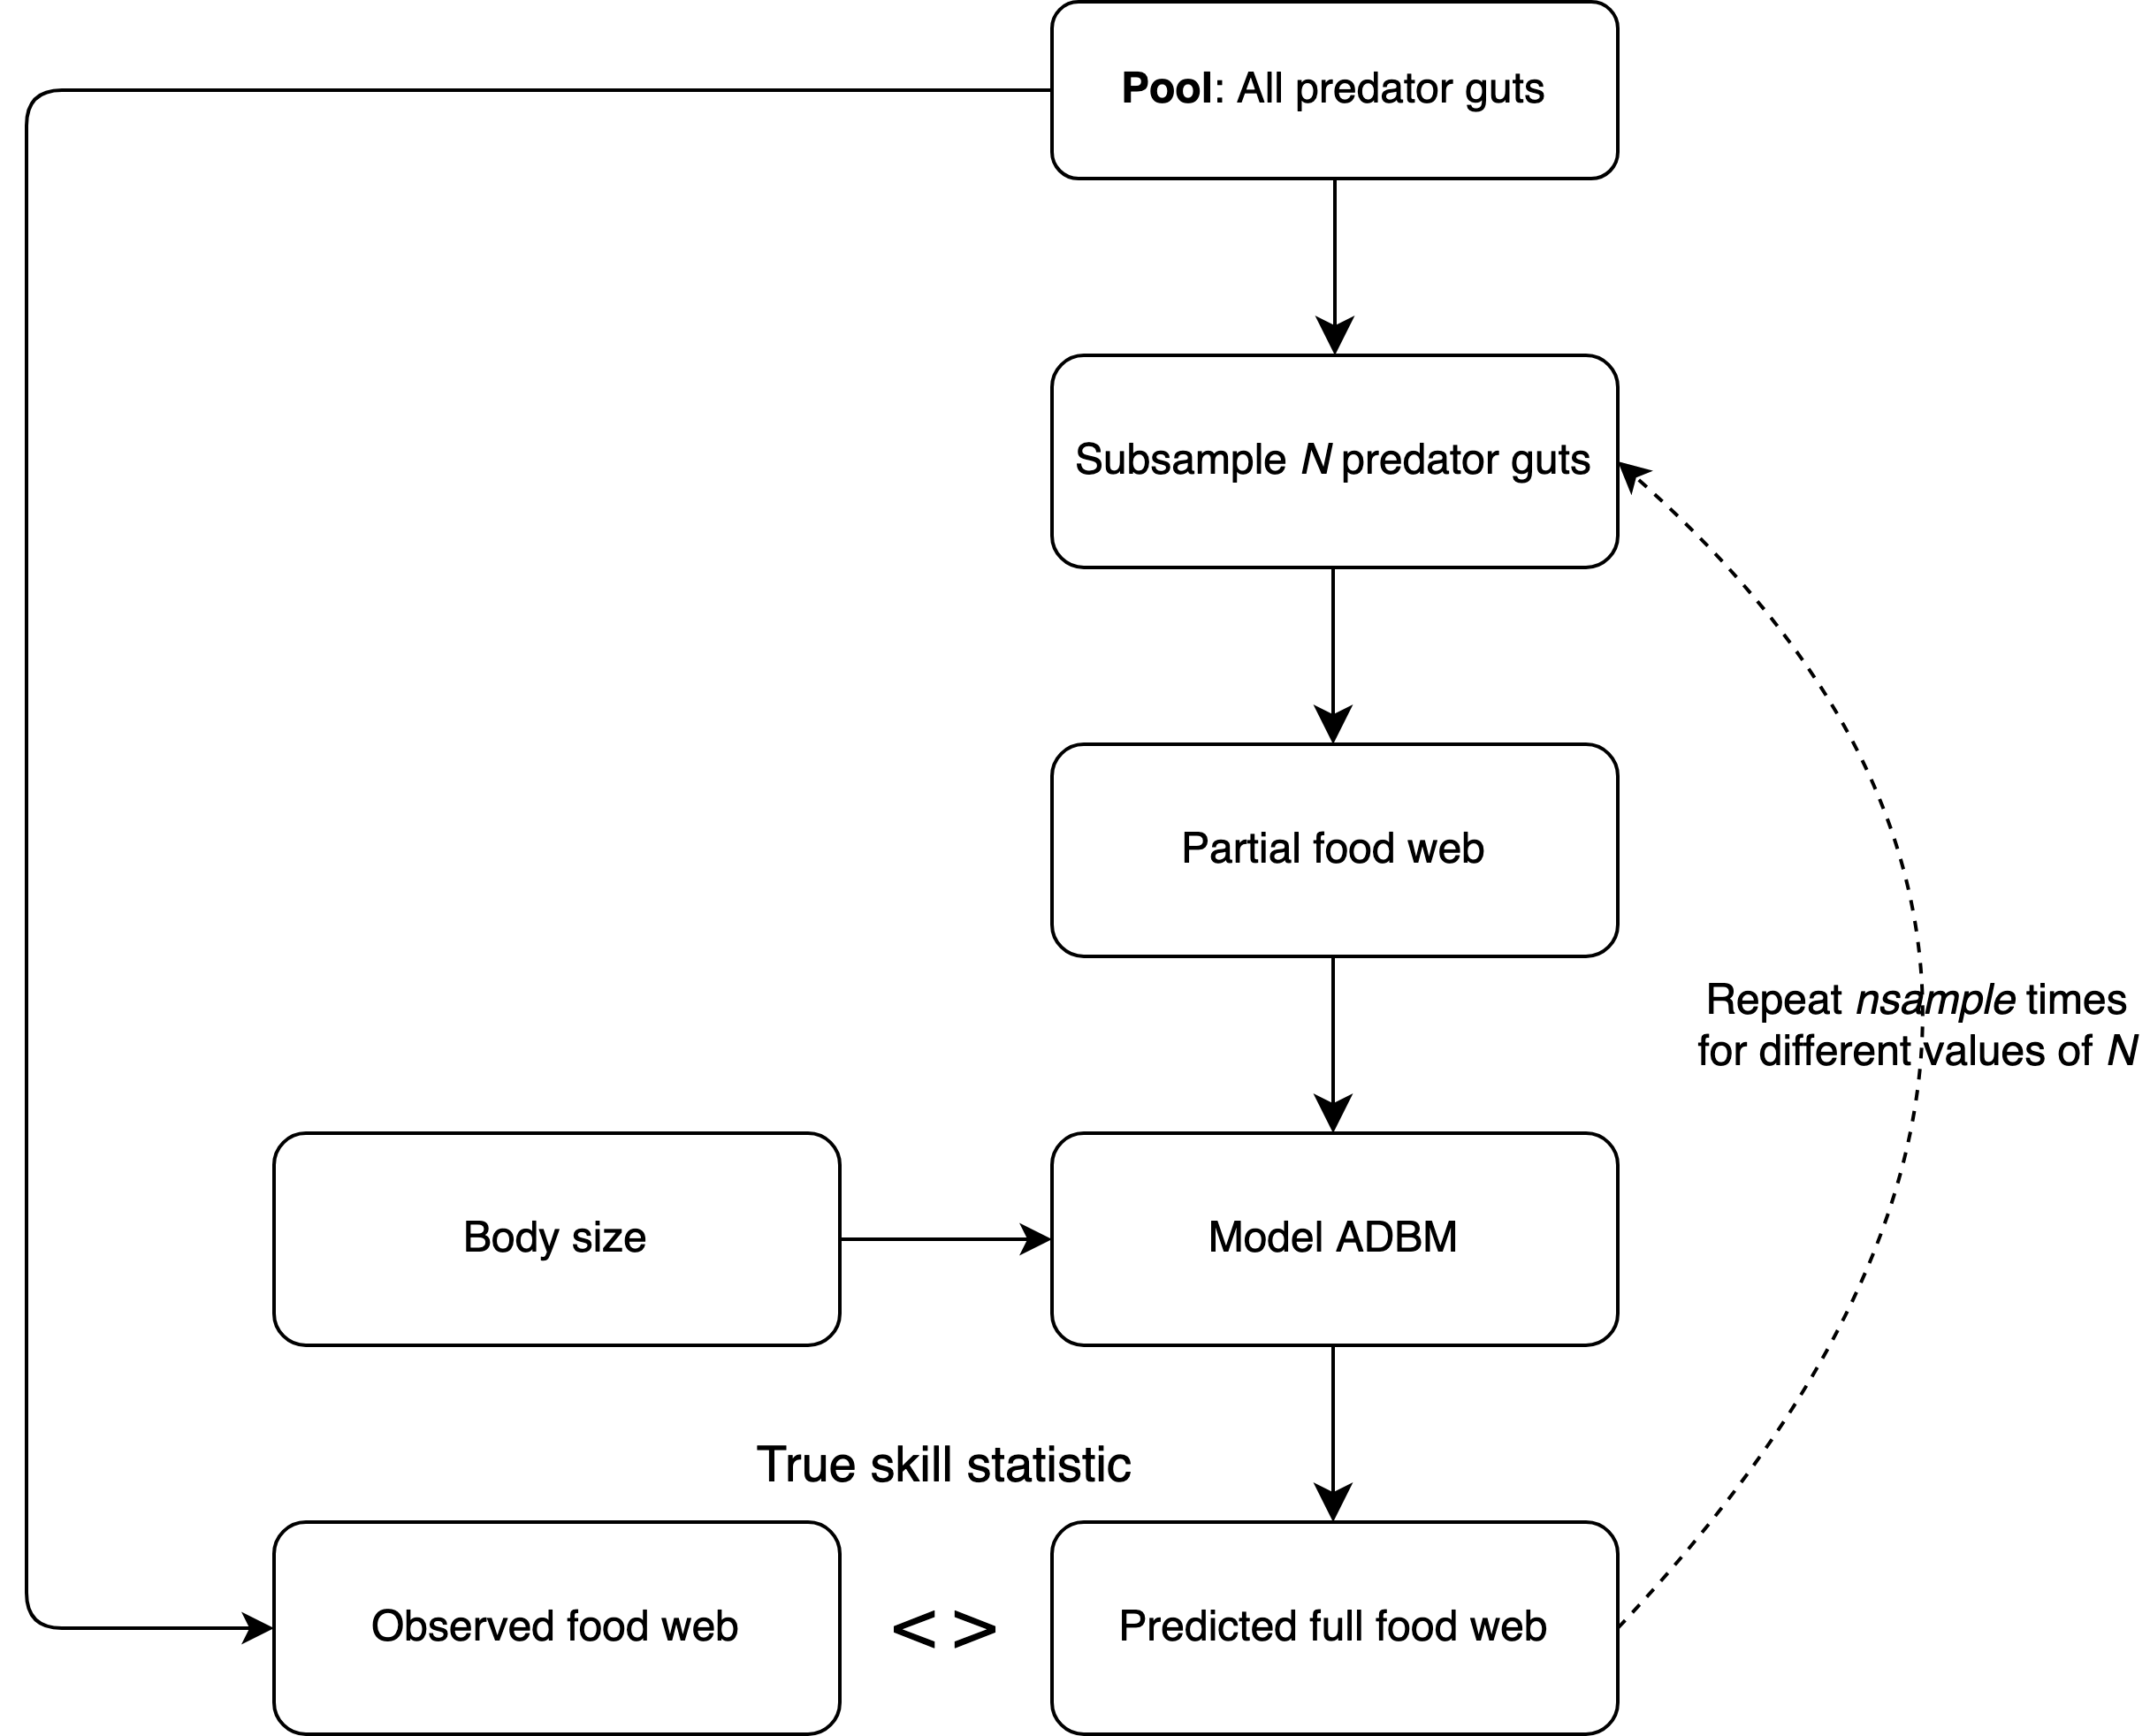
\includegraphics[width=350px]{../../manuscript/fig/ms_C2_flowchart} 

}

\caption{\label{fig:fig_ra} Flowchart of the subsampling method implemented to predict the full food web from the food web model using the predator guts.}\label{fig:unnamed-chunk-2}
\end{figure}

To fit the ADBM to partial predator guts dataset, we used the rejection
approximate Bayesian computation method we previously developed in
Gupta, Furrer, and Petchey (2022) to accept a parameter value from a
prior distribution which would have resulted in the minimum distance,
where distance = 1 - TSS. The true skill statistic was computed between
the diets predicted from the ADBM, and those observed in the sampled
predator guts. We repeated this process \(n~(= 100)\) times for every
\(i\) number of guts, where \(i\) lies between 1 and total number of
predator guts in the pool.

\emph{Input:}

\begin{itemize}
\item
  Predators \(P: P = \{p_1, p_2, \dots, p_k \}\)
\item
  A pool of predator guts \(G: G = \{g_1, g_2, \dots, g_n\}\), where
  \(g_{n}\) is the observed diet matrix containing ones and zeros.
\item
  A model prediction
  \(model(\theta): ADBM(\theta) = \{d_{p_1}, d_{p_1}, \dots, d_{p_k}\}\),
  where \(d_{p_k}\) is the predicted diet matrix of predator \(k\)
  containing ones and zeros.
\item
  A summary statistic \(s(x): s(x) \subseteq model(\theta)\), where
  \(s(x)\) is the diet of some or all of the predators.
\item
  A distance function \(d(x_i, y) : d(x_i,y) = 1 - TSS(x_i, y)\), which
  quantifies how close the observed diet is to the predicted diet of
  some or all of the predators.
\item
  An observed food web
  \(Y: Y = \{d_{p_1}', d_{p_1}', \dots, d_{p_k}'\}\), where \(d_{p_k}'\)
  is the observed diet matrix of predator \(k\) containing ones and
  zeros.
\end{itemize}

\emph{Sampling:}

for \(i = 1, \dots, tgut\) where \(tgut\) is the total number of
predator guts in the pool \(G\)

\begin{itemize}
\item
  for \(j = 1, \dots, nsample\) where \(nsample\) is the number of
  independent samples to be drawn

  \begin{itemize}
  \item
    Subsample a set of predator guts \(y = \{g_1, g_2, \dots, g_i\}\)
    from the pool of predator guts \(G\)
  \item
    for \(k = 1, \dots, npar\) where \(npar\) is the number of parameter
    values to be sampled

    \begin{itemize}
    \item
      Draw a set of parameter values \(\theta_k\) from the prior
      distribution \(\pi(\theta)\)
    \item
      Compute the model result \(x_k = model(\theta_k)\)
    \item
      Compute \(s(x_k)\) and \(d(s(x_k), y)\)
    \end{itemize}
  \item
    Accept \(\theta_j\), which results in the \(min_k\{d(s(x_k), y)\}\)
  \end{itemize}
\item
  Compute
  \(TSS_{i}(x, Y) = \{TSS(x_i, Y): x_i = ADBM(\theta_j), \theta_j \text{ computed from previous step}\}\)
  using the accepted \(\theta_1, \dots, \theta_{nsample}\)
\end{itemize}

\emph{Output:}

The \(TSS\) between observed and predicted food webs, and the posterior
parameter distributions for every \(i\) number of predator guts drawn
from the pool of predator guts.

\hypertarget{computing-the-minimum-number-of-predator-guts}{%
\subsection{Computing the minimum number of predator
guts}\label{computing-the-minimum-number-of-predator-guts}}

Using TSS of the model predicted food webs for different number of
predator guts, we computed the number of predator guts that results in
the mean TSS equal to the 95\% of the mean TSS achieved by the model
using all the predator guts available in the pool for a food web. We
call this number of predator guts as the minimum number of predator
guts.

\hypertarget{standardising-sampling-level-of-the-food-webs}{%
\subsection{Standardising sampling level of the food
webs}\label{standardising-sampling-level-of-the-food-webs}}

Since the seven food webs have different levels of sampling effort, with
Broadstone Stream being the most sampled among all, and every other food
web being undersampled when compared to the Broadstone Stream food web
(SI Fig. S2), we used the R \emph{vegan} package to account for the
undersampling with respect to the Broadstone Stream food web. We fitted
the link accumulation curves using the fitspecaccum function to a set of
nonlinear regression models suggested in Dengler (2009) and used the AIC
criteria for model selection. We then extrapolated the link accumulation
curves for all the food webs except the Broadstone Stream and computed
the corrected number of predator guts that would have resulted in the
gradient of the link accumulation curve equal to the gradient of that of
the Broadstone Stream when all the predator guts were used. We also
calculated the corrected number of trophic links corresponding to that
corrected number of predator guts. For the food webs, we calculated the
undersampling factor which is equal to the ratio of corrected number of
predator guts to the number of predator guts in the pool. Using the
undersampling factor, we further calculated the corrected minimum number
of predator guts which is equal to the product of the undersampling
factor and the minimum number of predator guts.

\hypertarget{results}{%
\section{Results}\label{results}}

We first present how the accuracy of the food web model in predicting
trophic interactions varies with increasing amount of predator guts
provided to the food web model. We investigate how the minimum number of
predator guts varied with number of trophic links and number of species.

\begin{figure}

{\centering 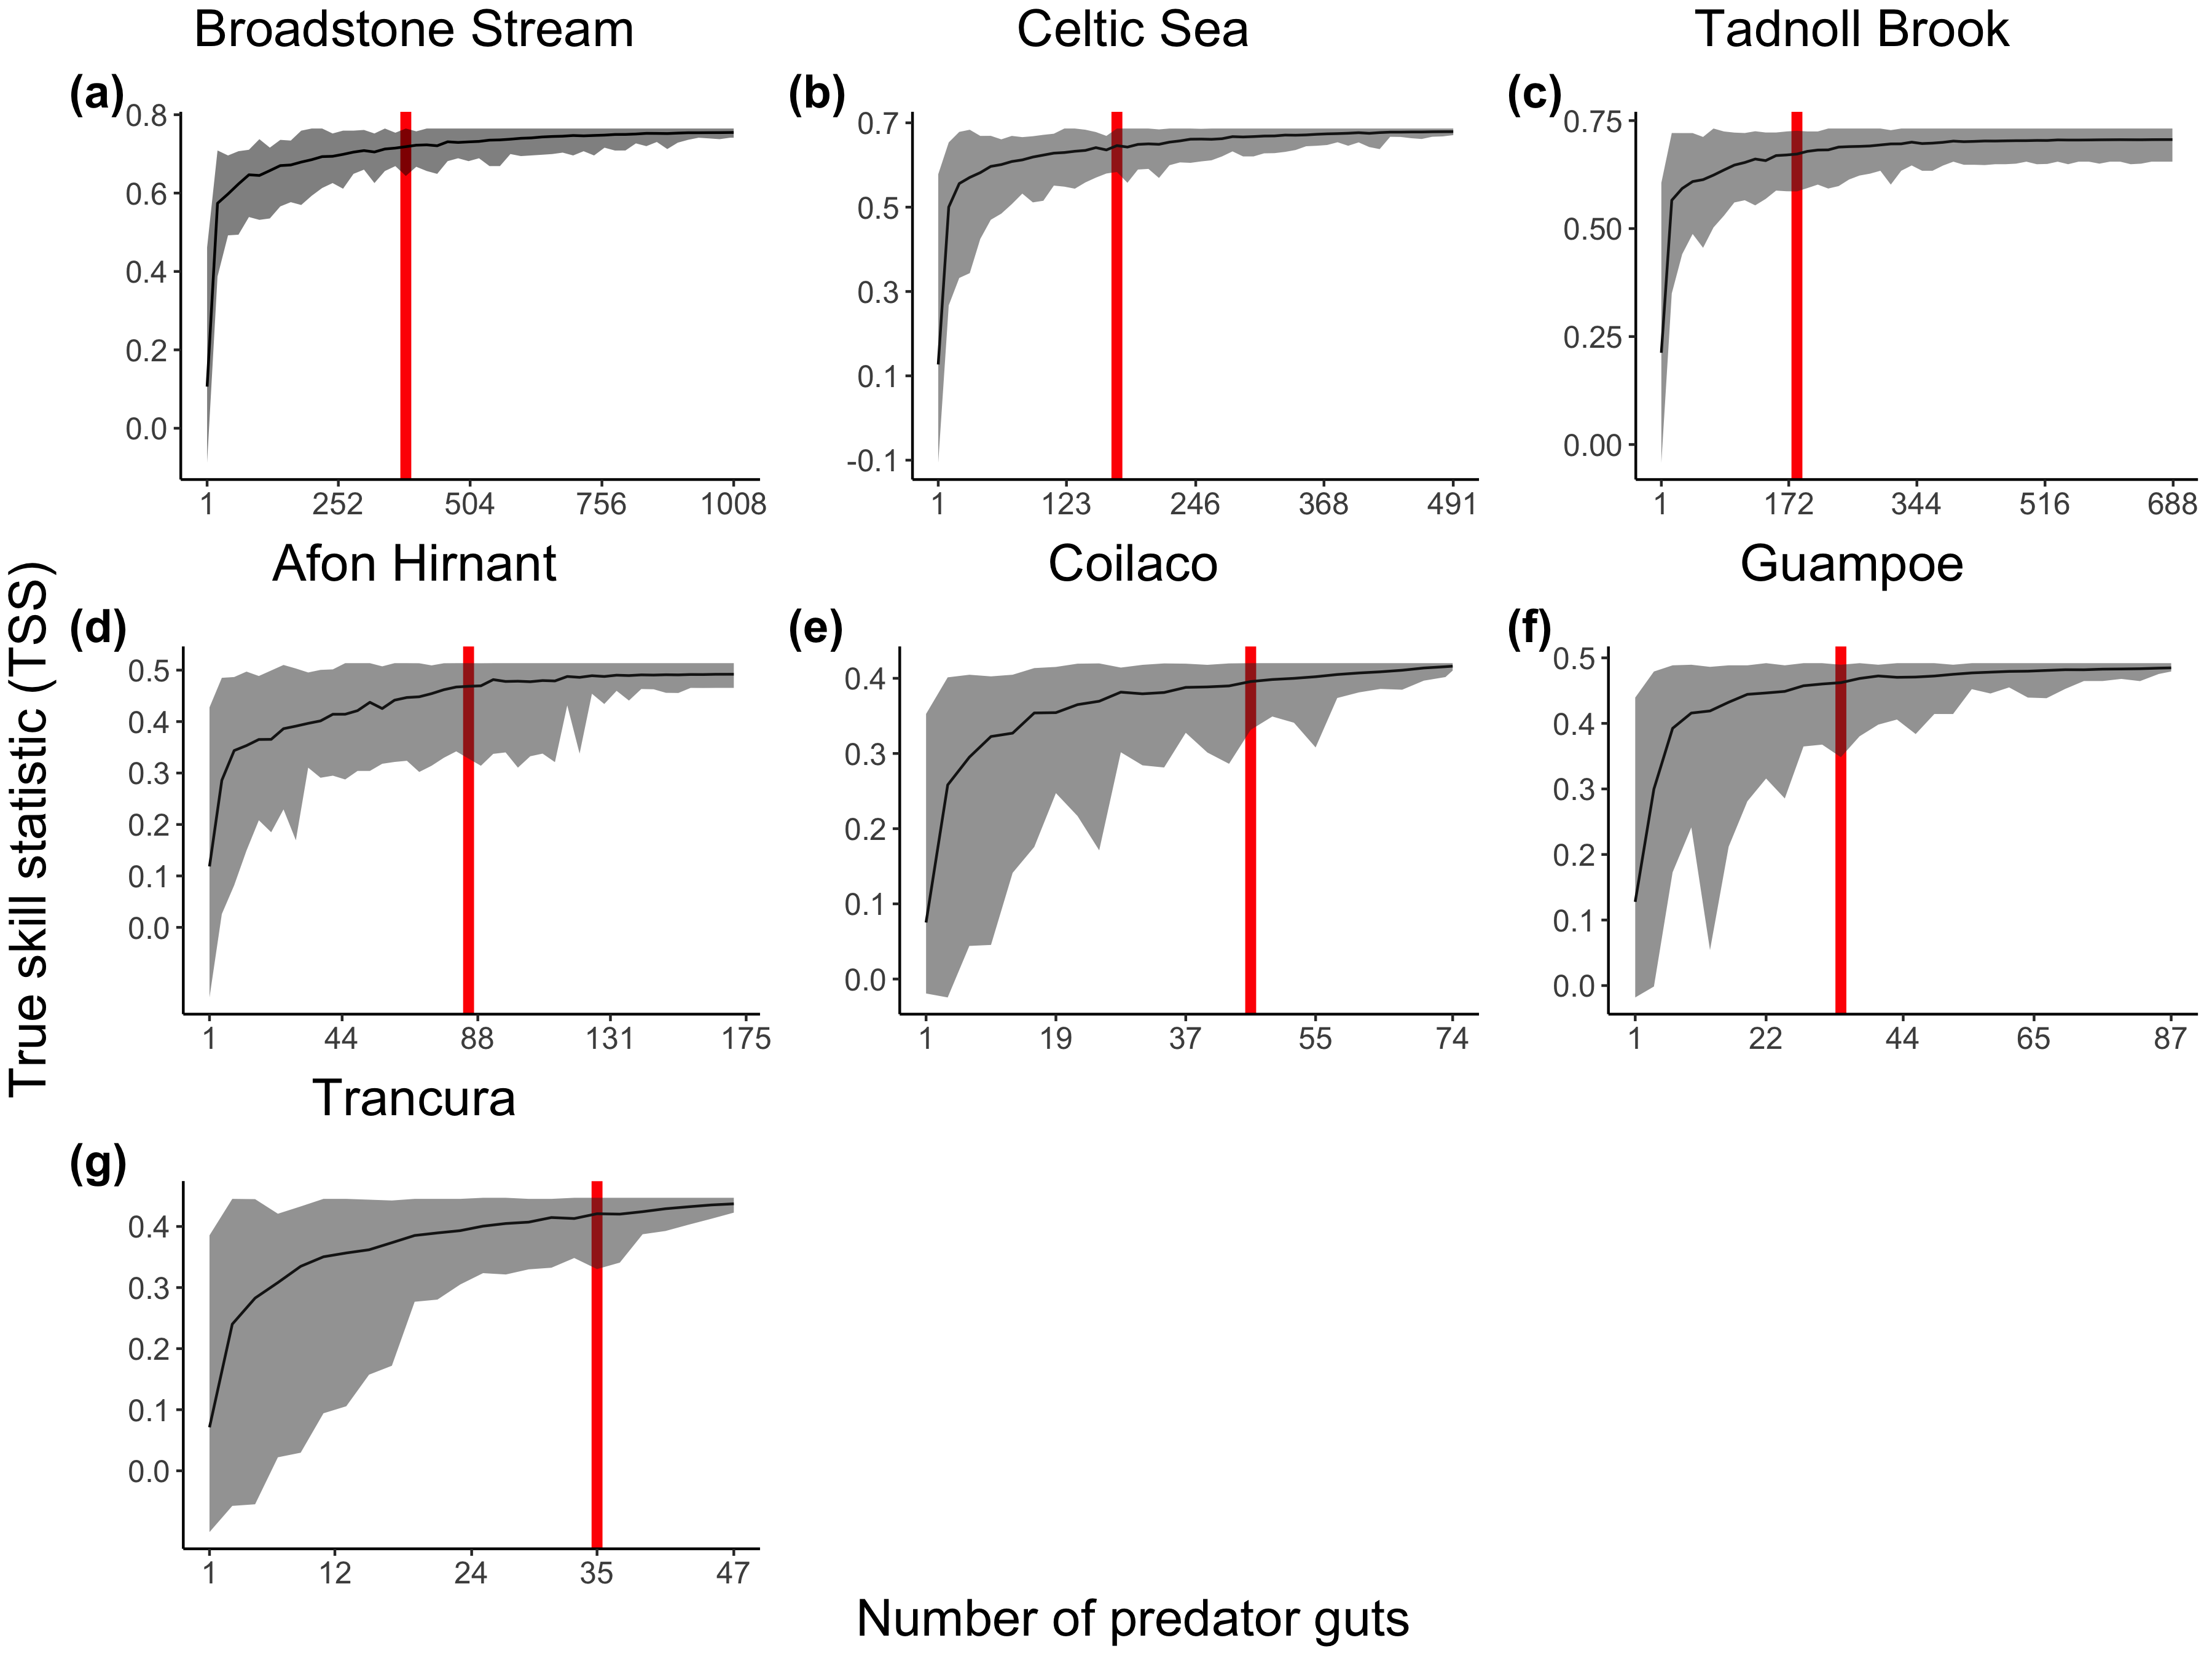
\includegraphics[width=400px]{../../results/misc/plot_TSS_vs_ngut} 

}

\caption{\label{fig:fig_ra} Accuracy of the predicted food web measured using the true skill statistic, predicted by the ADBM parameterised using predator guts. Line and shaded grey region represents the mean and the prediction interval corresponding to 100 independent samples respectively. Red line represents the number of predator guts required to achieve a TSS of 95\% of the maximum TSS.}\label{fig:unnamed-chunk-3}
\end{figure}

The true skill statistics of the food webs predicted by the ADBM using
incomplete predator guts improved quickly for lower number of predator
guts (Fig. \ref{fig:fig_ra}). Furthermore, the width of the prediction
interval of the true skill statistics decreased with increasing number
of predator guts with the mean TSS asymptoting to the maximum mean TSS
achieved by the ADBM when all the predator guts was used. Although the
maximum TSS varied among the food webs, the qualitative increase in the
TSS was the same.

For Broadstone Stream food web, with only 381 predator guts, which is
38\% of the total predator guts, the ADBM predicted the food web with
the mean TSS of 0.74. This was equivalent to 95\% of the mean TSS (0.78)
achieved using complete predator guts (Fig. \ref{fig:fig_ra}(a)):
i.e.~the main characteristics of the food web could be captured with
about 1/3 of the effort used in the original study. In case of the
Celtic Sea food web, only 171 predator guts which is 35\% of the total
predator guts was required by the ADBM to predict food web with TSS
equal to 95\% of the mean TSS (0.68) achieved using complete predator
guts (Fig. \ref{fig:fig_ra}(b)).

The minimum number of predator guts was not significantly related to
number of trophic links (Fig. \ref{fig:fig_rb} (a)) and the number of
species (Fig. \ref{fig:fig_rb} (b)). Similarly, the corrected minimum
number of predator guts was not significantly related to corrected
connectance, corrected number of trophic links and number of species
respectively (Fig. \ref{fig:fig_rb} (c, d)). Correcting for the
undersampling in the food webs improved the fit between the minimum
number of predator guts and the number of trophic links from
\(R^2 = 0.13\) (Fig. \ref{fig:fig_rb} (a)) to \(R^2 = 0.43\) (Fig.
\ref{fig:fig_rb} (c)).

\begin{figure}

{\centering 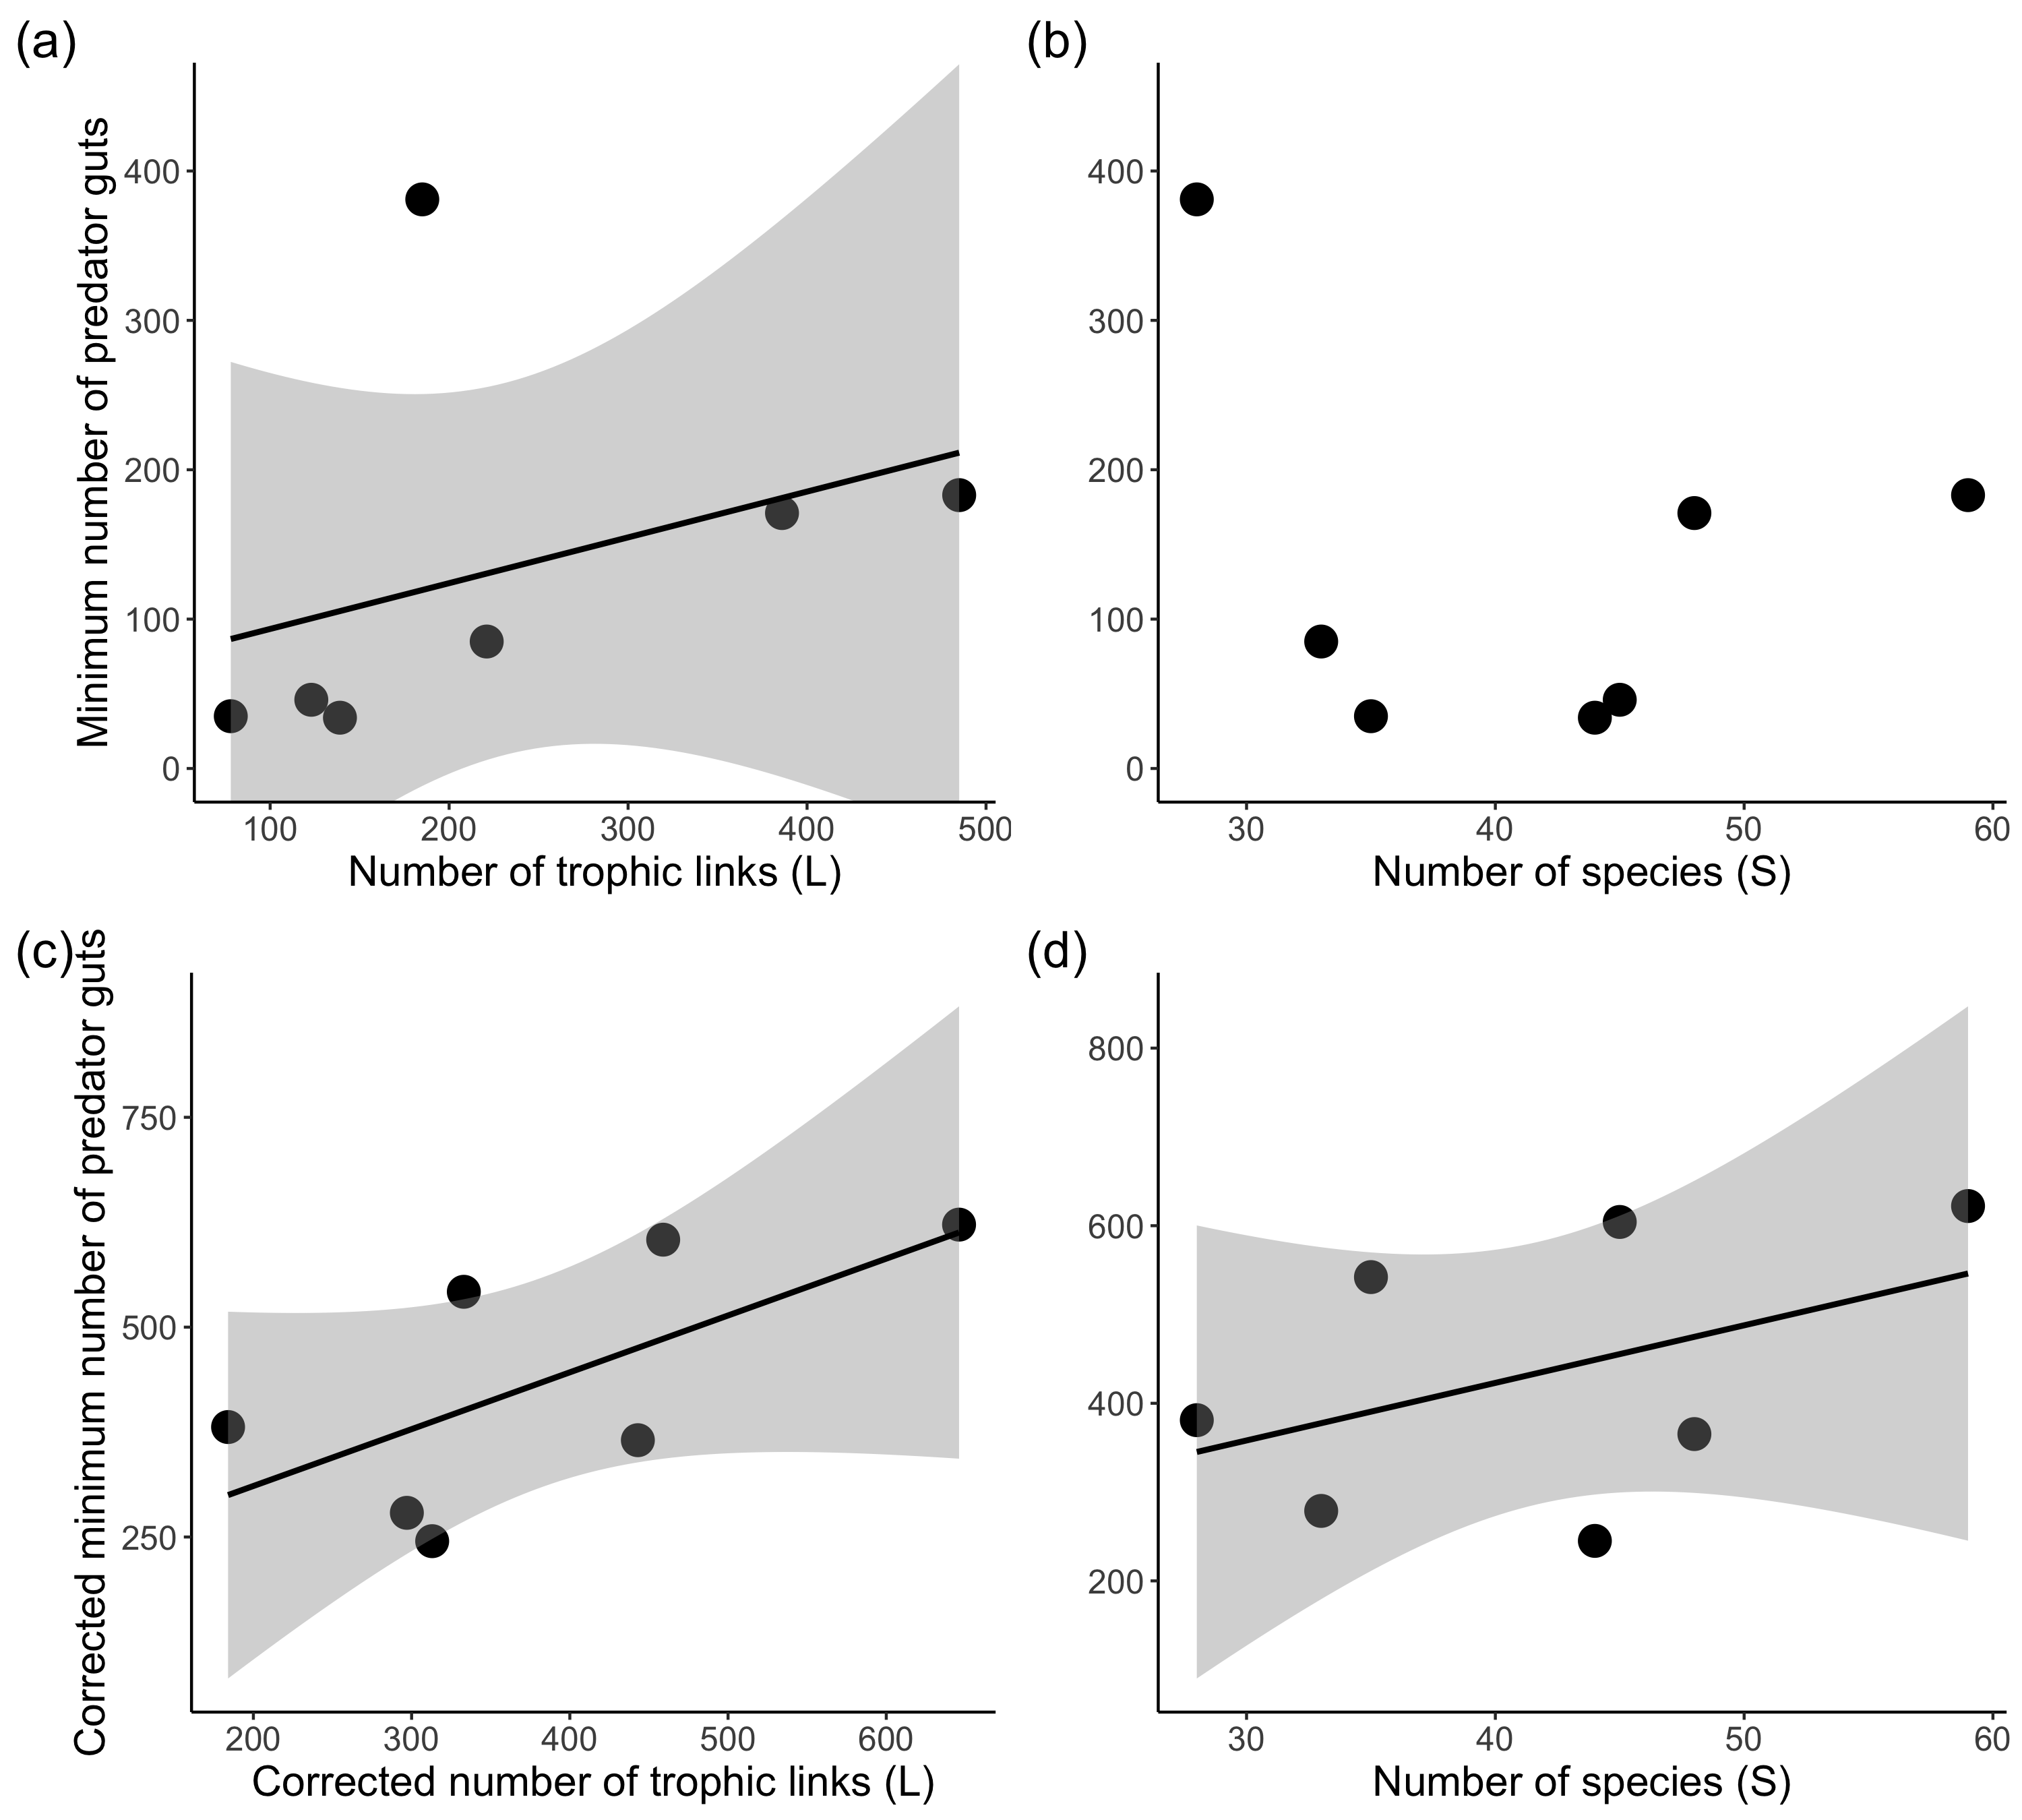
\includegraphics[width=300px]{../../results/misc/plot_n_min_gut_vs_SL} 

}

\caption{\label{fig:fig_rb} (a, b) Minimum number of predator guts (i.e the amount of predator guts used in order to ensure 95\% of the maximum TSS) plotted against number of trophic links (L) and number of species respectively. (c, d) Corrected minimum number of predator guts (i.e. the minimum number of predator guts which takes into account the undersampling level of the food webs) plotted against corrected number of trophic links and number of species (S) respectively. Solid lines are linear regression ((a) t = 0.876, df = 5, P = 0.421; (c) t = 1.923, df = 5, P = 0.113; (d) t = 1.099, df = 5, P = 0.322) and grey region represents 95\% confidence intervals.}\label{fig:unnamed-chunk-4}
\end{figure}

\hypertarget{discussion}{%
\section{Discussion}\label{discussion}}

We have demonstrated how a food web model can be used to predict the
full structure of a food web when incomplete data about trophic
interactions is available, which is true in most of the real food webs.
This can help inform how much predator guts to actually collect when we
are using a food web model to infer trophic interactions for an
ecosystem with a given number of species. A future development could be
to make the same assessment using other food web models, and to also use
food web data other than predator guts to parameterise those models.

Our study provides a ballpark figure of the minimum number of predator
guts that need to be sampled to predict the structure of a food web
using a food web model for an ecosystem with a given number of species.
For instance, Fig. \ref{fig:fig_rb} (d) can be used as a rough estimate
of how many predator guts needs to be collected to predict food web
structure using a food web model for a given number of species. This
would lead to a reduction in the hundreds of predator guts that would
have to be collected in the first place (Ings et al. 2009), thereby
saving considerable time and resources.

In our study, we have implemented the approach only with the ADBM, which
is a model based on size rules. Therefore, we suspect to get a similar
result (i.e.~minimum number of predator guts for a food web) for a
different food web model based on size rules such as the niche model by
Gravel et al. (2013). For a given food web, some food web models might
do better job at predicting its structure as compared to other food web
models, so we suggest to extend our approach to other food web models
such as niche model (Williams and Martinez 2000; Gravel et al. 2013;
Allesina, Alonso, and Pascual 2008) and nested hierarchical model
(Cattin et al. 2004). A future prospect could be to study how well
different food web models' prediction accuracy vary with different
amount of predator guts. This can also help in making decision as to
which food web model to chose from for a given a set of predator guts.
We suspect the relationship (i.e shape of the curve) between the TSS of
the predicted food web and the number of predator guts might vary within
food web models because of the difference on the set of rules used to
define those models and how well those rules explain the food web
structure. For example: a food web model based on body size trait would
require less amount of data to predict a size structured food web as
compared to a food web model based on trait other than body size.

Some studies have presented how the accuracy of food web prediction
change when the amount of food web data is varied (Gray et al. 2015b).
For example Desjardins-Proulx et al. (2017) has used predictive machine
learning models and Caron et al. (2022) has used predictive traits-based
models on partial knowledge of interactions to reconstruct a food web
accurately, in contrast to our study where we used a mechanistic food
web model.

In all of the seven food webs, the ADBM was able to infer the trophic
interactions using incomplete predator guts because the presence absence
information from the predator guts was still sufficient to constrain the
possible model parameter values of the ADBM that best explained the
predators' diets. Although in theory the ADBM can predict trophic
interactions using only body sizes of organisms as it is based on set of
foraging rules, it still requires some presence absence data to
constrain the posterior parameter space thereby making more accurate
predictions (Petchey et al. 2008).

To characterise trophic interactions which are rare in the nature one
would require more predator guts to observe those interactions as
compared to characterising trophic interactions which are more frequent
in the nature. The model is perhaps able to infer these rare
interactions using a relatively lower number of predator guts which one
might have inferred directly from the predator guts only after
collecting a large number of gut content samples.

Like any other food web models, the food web model used (the ADBM)
cannot explain all the interactions in any observed food web that it has
been fit to. The foraging rules it encodes are based on the body size
and have particular structure and assumptions; not all of these are met
by all observed interactions (Petchey et al. 2008). For example, the
ADBM can only predict diets that are contiguous with respect to the size
of prey. I.e. it cannot predict that a predator will consume organism of
size 1 and 3, and not organism of size 2. Hence, if the observed diets
are not contiguous when prey are ordered by their size, the estimation
process could lead to a lower value of the TSS (Gupta, Furrer, and
Petchey 2022).

Furthermore, the observed data may be missing links, e.g.~links that
rarely occur. Some of these food webs are undersampled (SI Fig. S2)
suggesting those food webs might be missing these rare trophic links,
and the false positives from a model might be a correctly predicted
link. A future prospect could be to incorporate other sources of
presence-absence data such as stable isotope ratio (Layman et al. 2007),
DNA metabarcoding (Roslin and Majaneva 2016), literature review (Gray et
al. 2015b; Cohen and Mulder 2014a; Goldwasser and Roughgarden 1993a) and
experimentation (Warren 1989) to complement any trophic links that were
missed by the gut content method.

We expected a positive relationship between the minimum number of
predator guts and the number of trophic links and number of species
respectively. However, we did not find such relation (Fig.
\ref{fig:fig_rb} (a, b)). We suspect this is due to the possibility that
the food webs are sampled at different level (SI Fig. S2), with
Broadstone Stream being the most sampled among all the food webs. Taking
into account the undersampling factor resulted in a better fit between
the corrected minimum number of predator guts and corrected number of
trophic links and number of species respectively (Fig. \ref{fig:fig_rb}
(c, d)), however did not result in a relationship. This could be due to
heterogenity in the predator guts across food webs and heterogenity
among food webs. First, if less number of prey items are present in a
predator gut then more number of predator guts would need to be
collected on an average to quantify the diet of that predator. Second, a
food web which has a high proportion of generalist species would require
a high number of predator guts on average to characterise the food web
structure as compared to characterising the structure of a food web
which has a high proportion of specialist species.

In our study, we have not considered uncertainty which is involved in
analysing the predator guts (Baker, Buckland, and Sheaves 2014). For
example, there are sometimes loose tissues that are not identifiable and
cannot be assigned to a specific prey item with certainty. There are
factors such as sample size of consumers, mechanical prey handling,
differential digestion and evacuation rates of different prey types and
volumes, and the ingestion order that in combination result in an
unquantifiable error which is difficult to interpret in the predator
diet (Hyslop 1980; Rindorf and Lewy 2004; Baker, Buckland, and Sheaves
2014). Therefore, the next step could be to incorporate these different
factors of uncertainty in parameterising the model and to understand how
these affect the accuracy of the predicted food webs.

\hypertarget{acknowledgements}{%
\section{Acknowledgements}\label{acknowledgements}}

This work was supported by the University Research Priority Program
Global Change and Biodiversity (Grant number: U-704-04-11) of the
University of Zurich. We thank the Petchey group members for their
valuable suggestions in the manuscript.

\hypertarget{author-contributions}{%
\section{Author contributions}\label{author-contributions}}

\hypertarget{reference}{%
\section*{Reference}\label{reference}}
\addcontentsline{toc}{section}{Reference}

\hypertarget{refs}{}
\begin{CSLReferences}{1}{0}
\leavevmode\vadjust pre{\hypertarget{ref-allesinaGeneralModelFood2008}{}}%
Allesina, Stefano, David Alonso, and Mercedes Pascual. 2008. {``A
{General Model} for {Food Web Structure}.''} \emph{Science} 320 (5876):
658--61. \url{https://doi.org/10.1126/science.1156269}.

\leavevmode\vadjust pre{\hypertarget{ref-alloucheAssessingAccuracySpecies2006}{}}%
Allouche, Omri, Asaf Tsoar, and Ronen Kadmon. 2006. {``Assessing the
Accuracy of Species Distribution Models: Prevalence, Kappa and the True
Skill Statistic ({TSS}).''} \emph{Journal of Applied Ecology} 43 (6):
1223--32. \url{https://doi.org/10.1111/j.1365-2664.2006.01214.x}.

\leavevmode\vadjust pre{\hypertarget{ref-bakerFishGutContent2014}{}}%
Baker, Ronald, Amanda Buckland, and Marcus Sheaves. 2014. {``Fish Gut
Content Analysis: Robust Measures of Diet Composition.''} \emph{Fish and
Fisheries} 15 (1): 170--77. \url{https://doi.org/10.1111/faf.12026}.

\leavevmode\vadjust pre{\hypertarget{ref-caronAddressingEltonianShortfall}{}}%
Caron, Dominique, Luigi Maiorano, Wilfried Thuiller, and Laura J.
Pollock. 2022. {``Addressing the {Eltonian} Shortfall with Trait-Based
Interaction Models.''} \emph{Ecology Letters} n/a (n/a).
\url{https://doi.org/10.1111/ele.13966}.

\leavevmode\vadjust pre{\hypertarget{ref-cattinPhylogeneticConstraintsAdaptation2004}{}}%
Cattin, Marie-France, Louis-F'elix Bersier, Carolin Banašek-Richter,
Richard Baltensperger, and Jean-Pierre Gabriel. 2004. {``Phylogenetic
Constraints and Adaptation Explain Food-Web Structure.''} \emph{Nature}
427 (6977, 6977): 835--39. \url{https://doi.org/10.1038/nature02327}.

\leavevmode\vadjust pre{\hypertarget{ref-cohenSoilInvertebratesChemistry2014}{}}%
Cohen, Joel E., and Christian Mulder. 2014a. {``Soil Invertebrates,
Chemistry, Weather, Human Management, and Edaphic Food Webs at 135 Sites
in {The Netherlands}: {SIZEWEB}.''} \emph{Ecology} 95 (2): 578--78.
\url{https://doi.org/10.1890/13-1337.1}.

\leavevmode\vadjust pre{\hypertarget{ref-cohen2014}{}}%
---------. 2014b. {``Soil Invertebrates, Chemistry, Weather, Human
Management, and Edaphic Food Webs at 135 Sites in The Netherlands:
SIZEWEB.''} \emph{Ecology} 95 (2): 578--78.
\url{https://doi.org/10.1890/13-1337.1}.

\leavevmode\vadjust pre{\hypertarget{ref-cohenStochasticTheoryCommunity1985}{}}%
Cohen, Joel E., C. M. Newman, and John Hyslop Steele. 1985. {``A
Stochastic Theory of Community Food Webs {I}. {Models} and Aggregated
Data.''} \emph{Proceedings of the Royal Society of London. Series B.
Biological Sciences} 224 (1237): 421--48.
\url{https://doi.org/10.1098/rspb.1985.0042}.

\leavevmode\vadjust pre{\hypertarget{ref-crawfordApplicationsStableIsotope2008}{}}%
Crawford, Kerry, Robbie A. Mcdonald, and Stuart Bearhop. 2008.
{``Applications of Stable Isotope Techniques to the Ecology of
Mammals.''} \emph{Mammal Review} 38 (1): 87--107.
\url{https://doi.org/10.1111/j.1365-2907.2008.00120.x}.

\leavevmode\vadjust pre{\hypertarget{ref-denglerWhichFunctionDescribes2009}{}}%
Dengler, Jürgen. 2009. {``Which Function Describes the Species--Area
Relationship Best? {A} Review and Empirical Evaluation.''} \emph{Journal
of Biogeography} 36 (4): 728--44.
\url{https://doi.org/10.1111/j.1365-2699.2008.02038.x}.

\leavevmode\vadjust pre{\hypertarget{ref-desjardins-proulxEcologicalInteractionsNetflix2017}{}}%
Desjardins-Proulx, Philippe, Idaline Laigle, Timoth'ee Poisot, and
Dominique Gravel. 2017. {``Ecological Interactions and the {Netflix}
Problem.''} \emph{PeerJ} 5 (August): e3644.
\url{https://doi.org/10.7717/peerj.3644}.

\leavevmode\vadjust pre{\hypertarget{ref-dunneNetworkStructureBiodiversity2002}{}}%
Dunne, Jennifer A., Richard J. Williams, and Neo D. Martinez. 2002.
{``Network Structure and Biodiversity Loss in Food Webs: Robustness
Increases with Connectance.''} \emph{Ecology Letters} 5 (4): 558--67.
\url{https://doi.org/10.1046/j.1461-0248.2002.00354.x}.

\leavevmode\vadjust pre{\hypertarget{ref-gilljamSeeingDouble2011}{}}%
Gilljam, David, Aaron Thierry, Francois K. Edwards, David Figueroa,
Anton T. Ibbotson, J. Iwan Jones, Rasmus B. Lauridsen, Owen L. Petchey,
Guy Woodward, and Bo Ebenman. 2011. {``Seeing {Double}:''} In
\emph{Advances in {Ecological Research}}, 45:67--133. {Elsevier}.
\url{https://doi.org/10.1016/B978-0-12-386475-8.00003-4}.

\leavevmode\vadjust pre{\hypertarget{ref-goldwasserConstructionAnalysisLarge1993a}{}}%
Goldwasser, Lloyd, and Jonathan Roughgarden. 1993a. {``Construction and
{Analysis} of a {Large Caribbean Food Web}.''} \emph{Ecology} 74 (4):
1216--33. \url{https://doi.org/10.2307/1940492}.

\leavevmode\vadjust pre{\hypertarget{ref-goldwasser1993}{}}%
---------. 1993b. {``Construction and Analysis of a Large Caribbean Food
Web.''} \emph{Ecology} 74 (4): 1216--33.
\url{https://doi.org/10.2307/1940492}.

\leavevmode\vadjust pre{\hypertarget{ref-gravelInferringFoodWeb2013}{}}%
Gravel, Dominique, Timoth'ee Poisot, Camille Albouy, Laure Velez, and
David Mouillot. 2013. {``Inferring Food Web Structure from Predator-Prey
Body Size Relationships.''} Edited by Robert Freckleton. \emph{Methods
in Ecology and Evolution} 4 (11): 1083--90.
\url{https://doi.org/10.1111/2041-210X.12103}.

\leavevmode\vadjust pre{\hypertarget{ref-grayJoiningDotsAutomated2015a}{}}%
Gray, Clare, David H. Figueroa, Lawrence N. Hudson, Athen Ma, Dan
Perkins, and Guy Woodward. 2015a. {``Joining the Dots: {An} Automated
Method for Constructing Food Webs from Compendia of Published
Interactions.''} \emph{Food Webs} 5 (December): 11--20.
\url{https://doi.org/10.1016/j.fooweb.2015.09.001}.

\leavevmode\vadjust pre{\hypertarget{ref-grayJoiningDotsAutomated2015}{}}%
---------. 2015b. {``Joining the Dots: {An} Automated Method for
Constructing Food Webs from Compendia of Published Interactions.''}
\emph{Food Webs} 5 (December): 11--20.
\url{https://doi.org/10.1016/j.fooweb.2015.09.001}.

\leavevmode\vadjust pre{\hypertarget{ref-guptaSimultaneouslyEstimatingFood2022}{}}%
Gupta, Anubhav, Reinhard Furrer, and Owen L. Petchey. 2022.
{``Simultaneously Estimating Food Web Connectance and Structure with
Uncertainty.''} \emph{Ecology and Evolution} 12 (3): e8643.
\url{https://doi.org/10.1002/ece3.8643}.

\leavevmode\vadjust pre{\hypertarget{ref-hattabForecastingFinescaleChanges2016}{}}%
Hattab, Tarek, Fabien Leprieur, Frida Ben Rais Lasram, Dominique Gravel,
François Le Loc'h, and Camille Albouy. 2016. {``Forecasting Fine-Scale
Changes in the Food-Web Structure of Coastal Marine Communities Under
Climate Change.''} \emph{Ecography} 39 (12): 1227--37.
\url{https://doi.org/10.1111/ecog.01937}.

\leavevmode\vadjust pre{\hypertarget{ref-hyslopStomachContentsAnalysis1980}{}}%
Hyslop, E. J. 1980. {``Stomach Contents Analysis---a Review of Methods
and Their Application.''} \emph{Journal of Fish Biology} 17 (4):
411--29. \url{https://doi.org/10.1111/j.1095-8649.1980.tb02775.x}.

\leavevmode\vadjust pre{\hypertarget{ref-ingsEcologicalNetworksFood2009}{}}%
Ings, Thomas C., Jos'e M. Montoya, Jordi Bascompte, Nico Blüthgen, Lee
Brown, Carsten F. Dormann, François Edwards, et al. 2009. {``Ecological
Networks--Beyond Food Webs.''} \emph{The Journal of Animal Ecology} 78
(1): 253--69. \url{https://doi.org/10.1111/j.1365-2656.2008.01460.x}.

\leavevmode\vadjust pre{\hypertarget{ref-jenningsPredictingEffectsClimate2010}{}}%
Jennings, Simon, and Keith Brander. 2010. {``Predicting the Effects of
Climate Change on Marine Communities and the Consequences for
Fisheries.''} \emph{Journal of Marine Systems} 79 (3-4): 418--26.
\url{https://doi.org/10.1016/j.jmarsys.2008.12.016}.

\leavevmode\vadjust pre{\hypertarget{ref-jenningsTrophicLevelsMarine2015}{}}%
Jennings, Simon, and Johan van der Molen. 2015. {``Trophic Levels of
Marine Consumers from Nitrogen Stable Isotope Analysis: Estimation and
Uncertainty.''} \emph{ICES Journal of Marine Science} 72 (8):
2289--2300. \url{https://doi.org/10.1093/icesjms/fsv120}.

\leavevmode\vadjust pre{\hypertarget{ref-jordanKeystoneSpeciesFood2009}{}}%
Jord'an, Ferenc. 2009. {``Keystone Species and Food Webs.''}
\emph{Philosophical Transactions of the Royal Society B: Biological
Sciences} 364 (1524): 1733--41.
\url{https://doi.org/10.1098/rstb.2008.0335}.

\leavevmode\vadjust pre{\hypertarget{ref-kadoyaIsoWebBayesianIsotope2012}{}}%
Kadoya, Taku, Yutaka Osada, and Gaku Takimoto. 2012. {``{IsoWeb}: {A
Bayesian Isotope Mixing Model} for {Diet Analysis} of the {Whole Food
Web}.''} Edited by Simon Thrush. \emph{PLoS ONE} 7 (7): e41057.
\url{https://doi.org/10.1371/journal.pone.0041057}.

\leavevmode\vadjust pre{\hypertarget{ref-kellyUsingEnvironmentalDNA2014}{}}%
Kelly, Ryan P., Jesse A. Port, Kevan M. Yamahara, and Larry B. Crowder.
2014. {``Using {Environmental DNA} to {Census Marine Fishes} in a {Large
Mesocosm}.''} \emph{PLOS ONE} 9 (1): e86175.
\url{https://doi.org/10.1371/journal.pone.0086175}.

\leavevmode\vadjust pre{\hypertarget{ref-laymanCanStableIsotope2007}{}}%
Layman, Craig A., D. Albrey Arrington, Carmen G. Montaña, and David M.
Post. 2007. {``Can {Stable Isotope Ratios Provide} for {Community}-{Wide
Measures} of {Trophic Structure}?''} \emph{Ecology} 88 (1): 42--48.
\url{https://doi.org/10.1890/0012-9658(2007)88\%5B42:CSIRPF\%5D2.0.CO;2}.

\leavevmode\vadjust pre{\hypertarget{ref-lindegrenEcologicalForecastingClimate2010}{}}%
Lindegren, Martin, Christian Möllmann, Anders Nielsen, Keith Brander,
Brian R. MacKenzie, and Nils Chr. Stenseth. 2010. {``Ecological
Forecasting Under Climate Change: The Case of {Baltic} Cod.''}
\emph{Proceedings of the Royal Society B: Biological Sciences} 277
(1691): 2121--30. \url{https://doi.org/10.1098/rspb.2010.0353}.

\leavevmode\vadjust pre{\hypertarget{ref-macarthurOptimalUsePatchy1966}{}}%
MacArthur, Robert H., and Eric R. Pianka. 1966. {``On {Optimal Use} of a
{Patchy Environment}.''} \emph{The American Naturalist} 100 (916):
603--9. \url{https://www.jstor.org/stable/2459298}.

\leavevmode\vadjust pre{\hypertarget{ref-nielsen2018}{}}%
Nielsen, Jens M., Elizabeth L. Clare, Brian Hayden, Michael T. Brett,
and Pavel Kratina. 2018. {``Diet Tracing in Ecology: Method Comparison
and Selection.''} Edited by M. Thomas P. Gilbert. \emph{Methods in
Ecology and Evolution} 9 (2): 278--91.
\url{https://doi.org/10.1111/2041-210X.12869}.

\leavevmode\vadjust pre{\hypertarget{ref-ogormanSimpleModelPredicts2019}{}}%
O'Gorman, Eoin J., Owen L. Petchey, Katy J. Faulkner, Bruno Gallo,
Timothy A. C. Gordon, Joana Neto-Cerejeira, J'on S. 'Olafsson, Doris E.
Pichler, Murray S. A. Thompson, and Guy Woodwar. 2019. {``A Simple Model
Predicts How Warming Simplifies Wild Food Webs.''} \emph{Nature Climate
Change} 9 (8, 8): 611--16.
\url{https://doi.org/10.1038/s41558-019-0513-x}.

\leavevmode\vadjust pre{\hypertarget{ref-peralta-maraverStructureDynamicsStability2017}{}}%
Peralta-Maraver, I., M. J. Lopez-Rodriguez, and J. M. Tierno de
Figueroa. 2017. {``Structure, Dynamics and Stability of a
{Mediterranean} River Food Web.''} \emph{Marine and Freshwater Research}
68 (3): 484--95. \url{https://doi.org/10.1071/MF15154}.

\leavevmode\vadjust pre{\hypertarget{ref-petcheySizeForagingFood2008}{}}%
Petchey, Owen L., Andrew P. Beckerman, Jens O. Riede, and Philip H.
Warren. 2008. {``Size, Foraging, and Food Web Structure.''}
\emph{Proceedings of the National Academy of Sciences} 105: 4191--96.
\url{https://doi.org/10.1073/pnas.0710672105}.

\leavevmode\vadjust pre{\hypertarget{ref-pompanonWhoEatingWhat2012}{}}%
Pompanon, Francois, Bruce E. Deagle, William O. C. Symondson, David S.
Brown, Simon N. Jarman, and Pierre Taberlet. 2012. {``Who Is Eating
What: Diet Assessment Using Next Generation Sequencing.''}
\emph{Molecular Ecology} 21 (8): 1931--50.
\url{https://doi.org/10.1111/j.1365-294X.2011.05403.x}.

\leavevmode\vadjust pre{\hypertarget{ref-rindorfBiasEstimatingFood2004}{}}%
Rindorf, A, and P Lewy. 2004. {``Bias in Estimating Food Consumption of
Fish by Stomach-Content Analysis''} 61: 12.

\leavevmode\vadjust pre{\hypertarget{ref-roslinUseDNABarcodes2016}{}}%
Roslin, Tomas, and Sanna Majaneva. 2016. {``The Use of {DNA} Barcodes in
Food Web Construction---Terrestrial and Aquatic Ecologists Unite!''}
Edited by Elizabeth Clare. \emph{Genome} 59 (9): 603--28.
\url{https://doi.org/10.1139/gen-2015-0229}.

\leavevmode\vadjust pre{\hypertarget{ref-tamaddoni-nezhadConstructionValidationFood2013}{}}%
Tamaddoni-Nezhad, Alireza, Ghazal Afroozi Milani, Alan Raybould, Stephen
Muggleton, and David A. Bohan. 2013. {``Construction and {Validation} of
{Food Webs Using Logic}-{Based Machine Learning} and {Text Mining}.''}
In \emph{Advances in {Ecological Research}}, 49:225--89. {Elsevier}.
\url{https://doi.org/10.1016/B978-0-12-420002-9.00004-4}.

\leavevmode\vadjust pre{\hypertarget{ref-wadaUseStableIsotopes1991}{}}%
Wada, E., H. Mizutani, and M. Minagawa. 1991. {``The Use of Stable
Isotopes for Food Web Analysis.''} \emph{Critical Reviews in Food
Science and Nutrition} 30 (4): 361--71.
\url{https://doi.org/10.1080/10408399109527547}.

\leavevmode\vadjust pre{\hypertarget{ref-warrenSpatialTemporalVariation1989}{}}%
Warren, Philip H. 1989. {``Spatial and {Temporal Variation} in the
{Structure} of a {Freshwater Food Web}.''} \emph{Oikos} 55 (3): 299.
\url{https://doi.org/10.2307/3565588}.

\leavevmode\vadjust pre{\hypertarget{ref-wilkinsonFAIRGuidingPrinciples2016}{}}%
Wilkinson, Mark D., Michel Dumontier, IJsbrand Jan Aalbersberg,
Gabrielle Appleton, Myles Axton, Arie Baak, Niklas Blomberg, et al.
2016. {``The {FAIR Guiding Principles} for Scientific Data Management
and Stewardship.''} \emph{Scientific Data} 3 (1, 1): 160018.
\url{https://doi.org/10.1038/sdata.2016.18}.

\leavevmode\vadjust pre{\hypertarget{ref-williamsSimpleRulesYield2000}{}}%
Williams, Richard J., and Neo D. Martinez. 2000. {``Simple Rules Yield
Complex Food Webs.''} \emph{Nature} 404 (6774, 6774): 180--83.
\url{https://doi.org/10.1038/35004572}.

\leavevmode\vadjust pre{\hypertarget{ref-woodward2010}{}}%
Woodward, Guy, Julia Blanchard, Rasmus B. Lauridsen, Francois K.
Edwards, J. Iwan Jones, David Figueroa, Philip H. Warren, and Owen L.
Petchey. 2010. {``Individual-Based Food Webs.''} In, 43:211--66.
Elsevier. \url{https://doi.org/10.1016/B978-0-12-385005-8.00006-X}.

\end{CSLReferences}

\bibliographystyle{biblatex}
\bibliography{bibliography.bib}


\end{document}
